\documentclass{article}
\usepackage[utf8]{inputenc}

\usepackage[margin=0.5in]{geometry}
\usepackage{parskip}

\usepackage{algorithm}
\usepackage{algpseudocodex}
\usepackage{amsmath}
\usepackage{amssymb}
\usepackage{amsthm}
\usepackage{enumerate}
\usepackage{enumitem}
\usepackage{mathtools}

\usepackage{hyperref}

\usepackage{float}

\newtheorem{lemma}{Lemma}
\newtheorem{theorem}{Theorem}

\DeclarePairedDelimiter{\parenthesesdelimiter}{(}{)}
\def\pars{\parenthesesdelimiter*}
\DeclarePairedDelimiter{\bracesdelimiter}{\{}{\}}
\def\braces{\bracesdelimiter*}
\let\set\braces
\DeclarePairedDelimiter{\bracketsdelimiter}{[}{]}
\def\brackets{\bracketsdelimiter*}
\DeclarePairedDelimiter{\lendelimiter}{|}{|}
\def\len{\lendelimiter*}

\DeclareMathOperator{\prob}{Pr}
\DeclareMathOperator{\expected}{\mathbb{E}}

\newcommand{\bigO}{\mathcal{O}}

\title{%
    Constructing an~MIS in Synchronous Graphs With Single Bit Messages\\%
    \normalsize based on\\%
    \large An optimal bit complexity randomized distributed MIS algorithm%
}
\author{Jakub Oskwarek}
\date{January 2024}

\begin{document}

\maketitle
\begin{abstract}
This project aims to understand the MIS construction algorithm proposed by Métivier, Robson, Saheb-Djahromi, and Zemmari, to outline the necessary intuitions and proofs for it, and to implement it in Go.
\end{abstract}

\section{Network properties}
The algorithm \cite{Metivier2011} is applicable to any graph, as long as the system adheres to the following assumptions:
\begin{itemize}
    \item Nodes \textbf{do not have identifiers} and are effectively indistinguishable. As an implementation detail, I~believe that seeding the local pseudorandom generators is a~reasonable exception to this rule.
    \item The algorithm proceeds in so-called \emph{bit rounds}, i.e. \textbf{synchronous rounds} in which the nodes exchange messages consisting of single bits.
    \item The communication channels are \textbf{fully reliable} --- bits are neither lost nor flipped in transmission.
\end{itemize}
We will be referring to the number of nodes as \(n\), but the algorithm does not have to know this value. In fact, the algorithm barely has to know anything. A~node only needs to be aware of which communication channel corresponds to which neighbor and to be able to draw random bits.

\section{An evolving idea}
In the original paper, the authors develop an algorithm that, with high probability, uses \(\bigO\pars{\log n}\) bit rounds. They recall other results concerning the coloring problem and its reduction to the MIS problem in order to draw the conclusion that their algorithm is optimal.

They start with an idealistic and intuitive approach.
\subsection{Algorithm \texorpdfstring{\(\mathcal{A}\)}{A}}
This will be a~greedy algorithm. The natural observation is that if we find a~strict local minimum in the graph (for some definition of a~``minimum'') and put it into the MIS once and for all, then this node's neighbors can never be in the MIS (by the very definition of the problem). So, once we put a~node into the MIS, we can ignore it and its neighbors in the operations that will follow.

Thus, the first algorithm proceeds in \emph{phases} as follows: in every \emph{phase}:
\begin{enumerate}
    \item Sample a~random number uniformly from \(\left[0, 1\right)\) --- this will be our criterion for the minimum
    \item Send this number to all neighbors
    \item Receive such number from all neighbors
    \item Now you know whether you are a~strict local minimum:
        \begin{itemize}
            \item if you are, then enter the MIS and announce it to all neighbors
            \item else, do not send anything
        \end{itemize}
    \item Receive analogous information from all neighbors
    \item Now you know whether you have a~neighbor in the MIS.
        \begin{itemize}
            \item if you do, then you will never have the chance to be in the MIS, so announce it to all neighbors
            \item else, do not send anything
        \end{itemize}
    \item Receive analogous information from all neighbors
    \item Now you know which neighbors can be ignored from now on:
        \begin{itemize}
            \item those already in the MIS
            \item those with no chance to enter
        \end{itemize}
        So, delete them.
\end{enumerate}
The node can finish processing when it knows its status in the MIS (definitely inside or definitely not).

There is a~problem: we wanted an algorithm that only sends single bit messages. All real numbers in \(\left[0, 1\right)\) are far from being representable with one bit. This calls for some improvement. Please give a~round of applause for

\subsection{Algorithm \texorpdfstring{\(\mathcal{B}\)}{B}}
It is a~simple modification of algorithm \(\mathcal{A}\) --- basically, it splits each phase into smaller parts and sends the sampled numbers bit by bit. A~node also exchanges some additional information about its status in the MIS. It allows everyone to keep track of which neighbors are in the MIS, which have no chance of entering in the current phase, and which have no chance of entering at all.

Each phase is accomplished by repeating these operations. When \(u\)~knows its status in the MIS or has no more active neighbors, it can break this loop and start another phase, if necessary, or terminate.

However, the next phase cannot always be started immediately because all the other vertices must be ready. A~question arises: is it really necessary? The answer is provided by

\subsection{Algorithm \texorpdfstring{\(\mathcal{C}\)}{C}}
Such delays are, in fact, not necessary. Instead of patiently waiting for the start of another phase, we can do some honest work during that time. In particular, if we, as a~node \(u\), have a~neighbor \(v\)~with whom we have already broken the symmetry for this phase, what is stopping us from attempting to break it in advance for the upcoming phases as well? Therefore, on a~given node, we will be running two alternating processes:
\begin{enumerate}
    \item perform a~round of symmetry breaking with the neighbors and remember the results --- they may (and probably will) refer to many different phases
    \item update the MIS status and announce the changes, if necessary
\end{enumerate}
At a~node \(u\), we will record three kinds of information, all represented by single bits:
\begin{itemize}
    \item \(\texttt{wins}\brackets{v}\brackets{p}\) --- whether we won against neighbor \(v\)~during the symmetry breaking for phase \(p\) (or undefined, if symmetry is yet to be broken with that neighbor for that phase)
    \item \(\texttt{ins}\brackets{v}\brackets{p}\) --- whether \(v\)~entered the MIS in phase \(p\) (or undefined, if not yet decided)
    \item \(\texttt{outs}\brackets{v}\brackets{p}\) --- whether \(v\)~was removed from the graph in phase \(p\) (or undefined, if not yet decided)
\end{itemize}
We will also maintain \(\texttt{win-phase}\brackets{v}\), \(\texttt{in-phase}\brackets{v}\), \(\texttt{out-phase}\brackets{v}\), and \(\texttt{index}[v]\), which will enable us to know at which phase we are with neighbor \(v\)~for each kind of information, and at which bit in that phase. The procedure \(b\pars{p, i}\) returns the \(i\)-th bit of the \(p\)-th phase by simply reading its value, if already sampled, or sampling it for the first time and recording it for future reference.

In the following code, \(N\)~will denote the set of \emph{all} neighbors, \(X\)~will denote the set of \emph{active} neighbors (i.e. those who have not yet decided to exclude themselves from the graph at any phase), and \(P\) will denote the current phase considered by the second process.
\begin{algorithm}[H]
\caption{A~logical round of algorithm \(\mathcal{C}\) (composed of three physical send-receive rounds) at a~node \(u\)}
\begin{algorithmic}
\LComment{Perform a~round of symmetry breaking}
\For{\(v \in X\)}
    \State send \(b\pars{\texttt{win-phase}\brackets{v}, \texttt{index}\brackets{v}}\) to \(v\) \Comment{send the next bit for the appropriate phase}
\EndFor
\For{\(v \in X\)}
    \State receive \(b_v\) from \(v\)
    \If{\(b_v \neq b\pars{\texttt{win-phase}\brackets{v}, \texttt{index}\brackets{v}}\)}
        \State \(\texttt{wins}\brackets{v}\brackets{\texttt{phase}\brackets{v}} \gets \brackets{b\pars{\texttt{win-phase}\brackets{v}, \texttt{index}\brackets{v}} = 0}\) \Comment{the symmetry is broken and we win if we sent a~zero}
        \State \(\texttt{win-phase}\brackets{v} \gets \texttt{win-phase}\brackets{v} + 1\) \Comment{we can start the symmetry breaking for another phase}
        \State \(\texttt{index}\brackets{v} \gets 0\) \Comment{we will, naturally, start that next phase from the beginning}
    \Else
        \State \(\texttt{index}\brackets{v} \gets \texttt{index}\brackets{v} + 1\) \Comment{the symmetry is not broken and we will need to exchange another bit}
    \EndIf
\EndFor
\LComment{Check whether we have enough information to decide if we enter the MIS}
\If{\(\forall_{v \in N}\texttt{wins}\brackets{v}\brackets{P} \neq \bot \land \textrm{not already decided for phase \(P\)}\)} 
    \For{\(v \in X\)}
        \State \(i \gets \brackets{\forall_{v \in N}\texttt{wins}\brackets{v}\brackets{P} = 1}\) \Comment{we enter the MIS if we won against all our neighbors}
        \State send \(i\)~to \(v\)
        \If{\(i = 1\)}
            \State enter the MIS
        \EndIf
    \EndFor
\EndIf
\For{\(v \in X\)}
    \State receive \(i_v\) from \(v\)
    \If{\(i_v \neq \bot\)}
        \State \(\texttt{ins}\brackets{v}\brackets{\texttt{in-phase}\brackets{v}} \gets i_v\)
        \State \(\texttt{in-phase}\brackets{v} \gets \texttt{in-phase}\brackets{v} + 1\)
    \EndIf
\EndFor
\LComment{Check whether we have enough information to decide if we should be deleted}
\If{\(\forall_{v \in N}\texttt{ins}\brackets{v}\brackets{P} \neq \bot \land \textrm{not already decided for phase \(P\)}\)}
    \State \(o \gets \exists_{v \in N}\texttt{ins}\brackets{v}\brackets{P} = 1 \lor \textrm{we are in the MIS}\)
    \For{\(v \in X\)}
        \State send \(o\)~to \(v\)
    \EndFor
    \If{\(o = 1\)}
        \State terminate when the round is completed
    \EndIf
\EndIf
\For{\(v \in X\)}
    \State receive \(o_v\) from \(v\)
    \If{\(o_v \neq \bot\)}
        \State \(\texttt{outs}\brackets{v}\brackets{\texttt{out-phase}\brackets{v}} \gets o_v\)
        \State \(\texttt{out-phase}\brackets{v} \gets \texttt{out-phase}\brackets{v} + 1\)
        \If{\(o_v = 1\)}
            \State \(X \gets X \setminus \set{v}\) \Comment{neighbor \(v\)~has decided to be removed from the graph}
        \EndIf
    \EndIf
\EndFor
\LComment{Try to advance to the next phase}
\If{\(\forall_{v \in N}\texttt{outs}\brackets{v}\brackets{P} \neq \bot\)}
    \State \(N \gets \set{v \in N : \texttt{outs}\brackets{v}\brackets{P} = 0}\) \Comment{keep only the neighbors that were not disconnected in phase \(P\)}
    \State \(P \gets P + 1\)
\EndIf

\end{algorithmic}
\end{algorithm}

This is the final version of the algorithm.

\section{Intuitions about correctness}
Let us, for a~moment, ``tune out'' the interspersed rounds of symmetry breaking and only look at these decisions of algorithm \(\mathcal{C}\)~that update the contents of the independent set or the ``shape'' of the graph, in a~per-phase manner.

The probability that algorithm \(\mathcal{C}\)~will go on forever is zero. To see that, let us look at a~phase that terminates. Each of the bit strings generated by the nodes for this phase represents the binary expansion of some~number \(r \in \left[0, 1\right)\). Let us pick a~node \(u\) that generated the bit string corresponding to the smallest of such numbers. This node cannot have a~neighbor with the same bit string because in such scenario the phase would not have terminated. Thus, \(u\)~is a~local minimum, so it will enter the set and exclude itself from the graph. Therefore, with each phase that terminates, the number of nodes in the graph decreases. Since \(n\)~is finite (which is not explicitly stated in the original paper, but it seems like a~fair assumption), in order to go on forever, algorithm \(\mathcal{C}\)~would need some phase to never terminate. However, the probability of such event is zero because it would require a~pair of nodes to generate identical infinite bit strings. 

 Now, let us investigate, how algorithm \(\mathcal{C}\)~makes its decisions. In every phase, it waits for the symmetry to be broken and only then does it decide whether a~node should enter the MIS. Then it waits for all the messages carrying such decisions in order to decide whether it should be excluded, and then it waits for all such messages in order to update its local ``vision'' of the graph. Thus, we can think of algorithm \(\mathcal{C}\) as making decisions consistent with those that \(\mathcal{A}\)~would make if, for each phase, it sampled the real numbers corresponding to the bit strings that \(\mathcal{C}\)~saw.

On the other hand, it is easy to see that algorithm \(\mathcal{A}\)~constructs a~valid independent set --- there can never be more than one strict local minimum, so no two adjacent nodes will ever end up together in the resulting collection in the same phase. They cannot enter the set in different phases either --- once the first one becomes a~member of the collection, the other one is immediately excluded from the graph. 

The set constructed by \(\mathcal{A}\)~is also maximal because the only way to terminate without being chosen as a~member of the constructed collection is to receive a~signal that a~neighbor has entered this collection.

Thus, we know that \(\mathcal{C}\)~constructs an~MIS.

\section{Proof of complexity (outline)}
\begin{lemma}
\label{lemma:A:phases}
With probability \(1 - o\pars{\frac{1}{n}}\), algorithm \(\mathcal{A}\)~needs \(\bigO\pars{\log n}\) phases.
\end{lemma}
\begin{proof}
Firstly, let us prove that, in expectation, the number of edges in the graph is halved in every phase. To do that, let us consider situations in which a~node \(u\)~samples the smallest number among the nodes \(N\pars{u} \cup N\pars{v}\), for some \(v \in N\pars{u}\). The probability of such event is at least
\begin{equation*}
    \frac{1}{\deg\pars{u} + \deg\pars{v}}
\end{equation*}
as it roughly corresponds to taking the first spot in a~sorted sequence of \(\deg\pars{u} + \deg\pars{v}\) numbers. Then, \(u\)~will become the local minimum and remove \(v\)~together with its \(\deg\pars{v}\) edges. By linearity of expectation, the expected number of edges that disappear in such situations is
\begin{equation*}
    \begin{split}
        \frac{1}{2}\sum_{\set{x, y} \in E}&\pars{\deg\pars{x} \cdot \prob\pars{\text{\(y\) removes \(x\) and all its edges}} + \deg\pars{y} \cdot \prob\pars{\text{\(x\) removes \(y\) and all its edges}}}\\
            &= \frac{1}{2}\sum_{\set{x, y} \in E}\pars{\deg\pars{x} \cdot \frac{1}{\deg\pars{x} + \deg\pars{y}} + \deg\pars{y} \cdot \frac{1}{\deg\pars{x} + \deg\pars{y}}}
            = \frac{1}{2}\sum_{\set{x, y} \in E}1
            = \frac{\len{E}}{2}
    \end{split}
\end{equation*}
The lemma follows from choosing a~constant \(a\)~such that after \(a\log n\) phases the expected number of edges is \(o\pars{\frac{1}{n}}\). In the paper, \(a = 4\) is deemed sufficient.
\end{proof}
\begin{lemma}
\label{lemma:C:phases}
In algorithm \(\mathcal{C}\), over a~single edge, symmetry is broken for \(a\log n\) phases in \(\bigO\pars{\log n}\) rounds with probability \(1 - o\pars{\frac{1}{n^3}}\).
\end{lemma}
\begin{proof}
The rounds are independent Bernoulli trials --- each one breaks the symmetry with probability \(\frac{1}{2}\). Assume that we have \(r\)~rounds. Let \(W\) be the number of \(\texttt{wins}\) resolved during those \(r\)~rounds. We have
\begin{equation*}
    \mu = \expected\brackets{W} = \frac{r}{2}
\end{equation*}
The lemma is then proven by plugging its statement, together with the above observation, into Chernoff's inequality and solving for all the necessary constants.
\end{proof}
\begin{theorem}
\label{theorem:C}
Algorithm \(\mathcal{C}\) terminates in \(\bigO\pars{\log n}\) rounds with probability \(1 - o\pars{\frac{1}{n}}\)
\end{theorem}
\begin{proof}
Since there are \(\bigO\pars{n^2}\) edges, then by lemma \ref{lemma:C:phases} and the union bound, the probability that there exists an edge over which the symmetry was broken fewer than \(a\log n\) times is \(o\pars{\frac{1}{n}}\). The number of rounds in the second process of algorithm \(\mathcal{C}\) is bounded by a~constant factor times the number of rounds in the first process. By lemma \ref{lemma:A:phases}, only \(a\log n\) phases are needed with probability \(1 - o\pars{\frac{1}{n}}\). Combining all that proves the desired property.
\end{proof}
\section{Remarks}
The exact way in which the two processes of algorithm \(\mathcal{C}\) alternate was not entirely clear to me.
\begin{enumerate}
    \item In my implementation, many bit exchange phases are processed concurrently. However, the second process is only concerned with one phase at a~time. I~do not know, how it could be made concurrent. I~believe that it would bring catastrophic consequences, e.g. a~node entering the set in anticipation, only to learn that it should have been deleted some phases earlier. However, the paper does not clearly reject that option.
    \item Currently, the logical rounds are organized in triplets: win --- in --- out. Probably, they could also be organized in quadruplets: win --- in --- win --- out. This might be in closer correspondence with the paper's original phrasing: one round of each process. However, I~believe that this only has the potential to shave off a~constant.
\end{enumerate}
Despite all those doubts, I~believe that my implementation is correct, i.e. \(\bigO\pars{\log n}\) and not \(\bigO\pars{\log^2n}\). For \(n\) up to \(350\), the average number of rounds seems to match the logarithmic curve with an empirically adjusted constant equal to \(7.1\).
\begin{figure}[H]
    \centering
    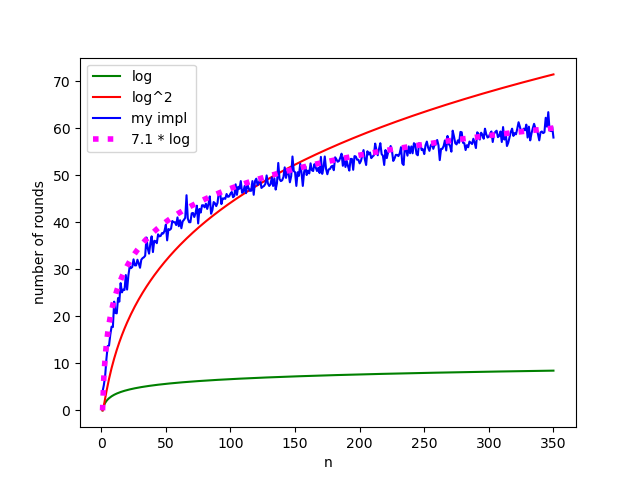
\includegraphics{comparison.png}
\end{figure}

\bibliographystyle{plain}
\bibliography{biblio.bib}

\end{document}
